

\begin{figure}[H]
  \centering
  \begin{tabular}{cc}
    \subfloat[Average number of cars in front of ego-vehicle.]{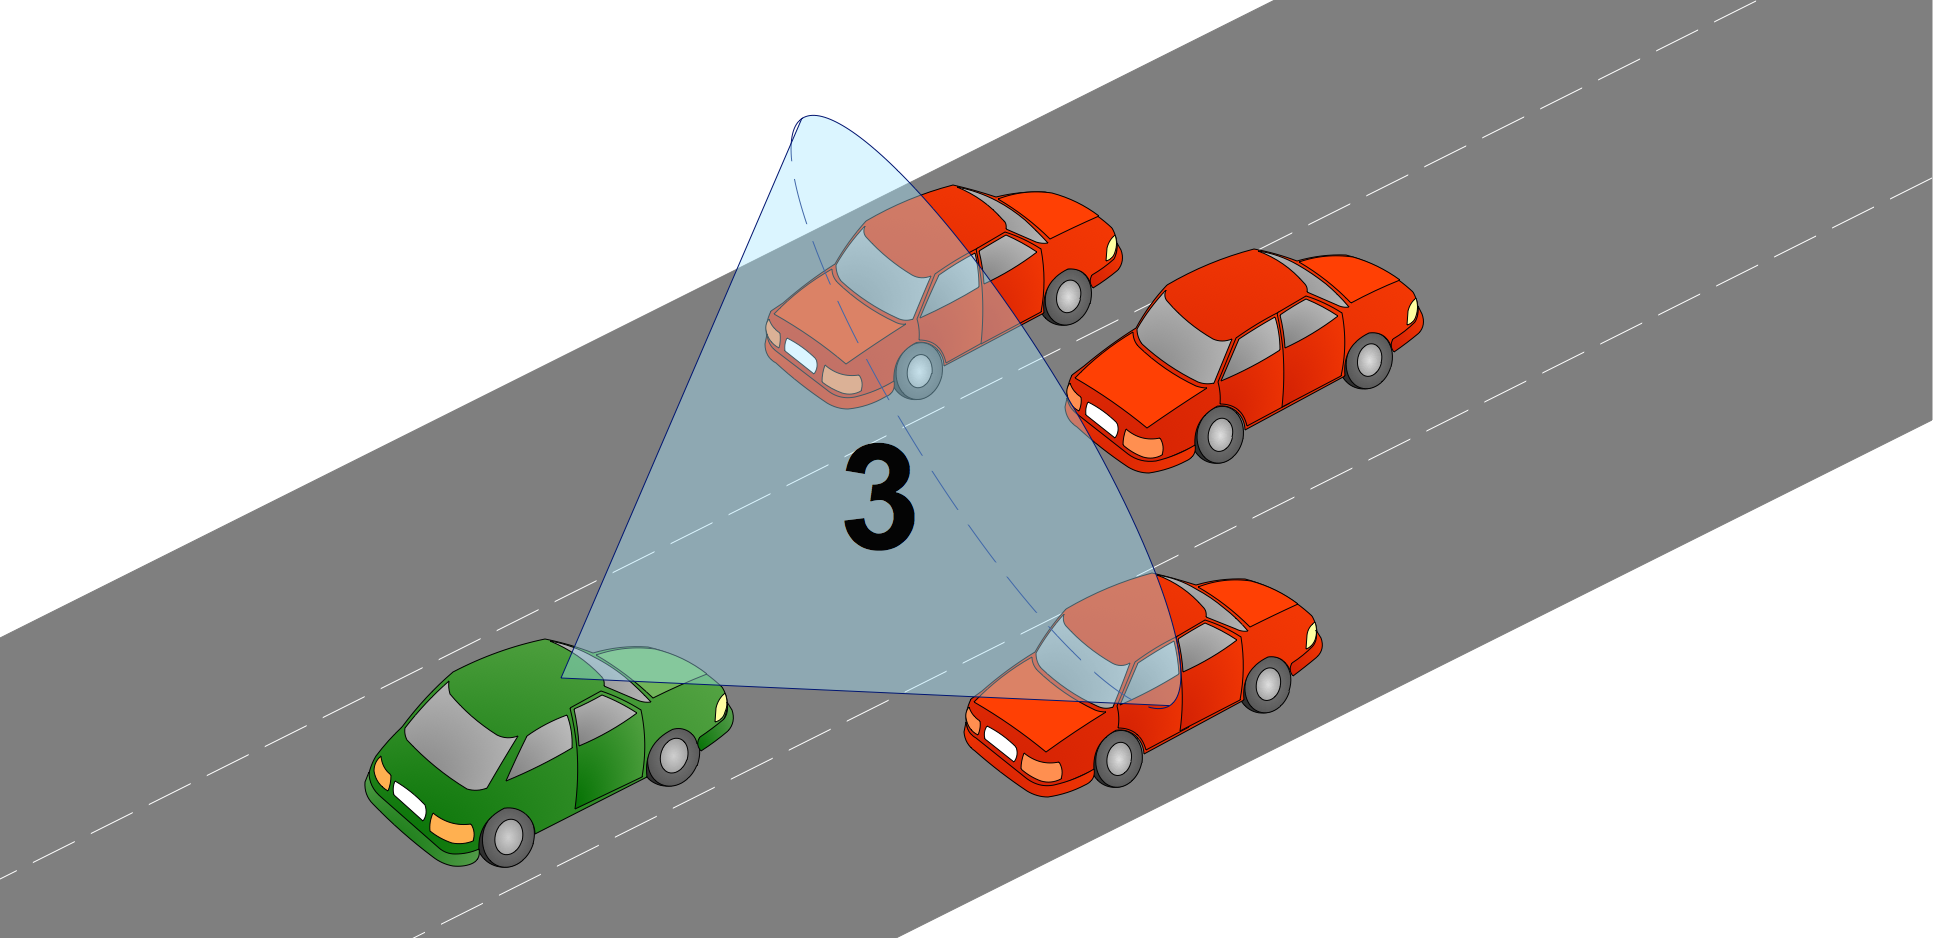
\includegraphics[width=0.45\textwidth]{text/figures/numOfObjects.png}} &
    \subfloat[Distance to rear-end of vehicle directly in front.]{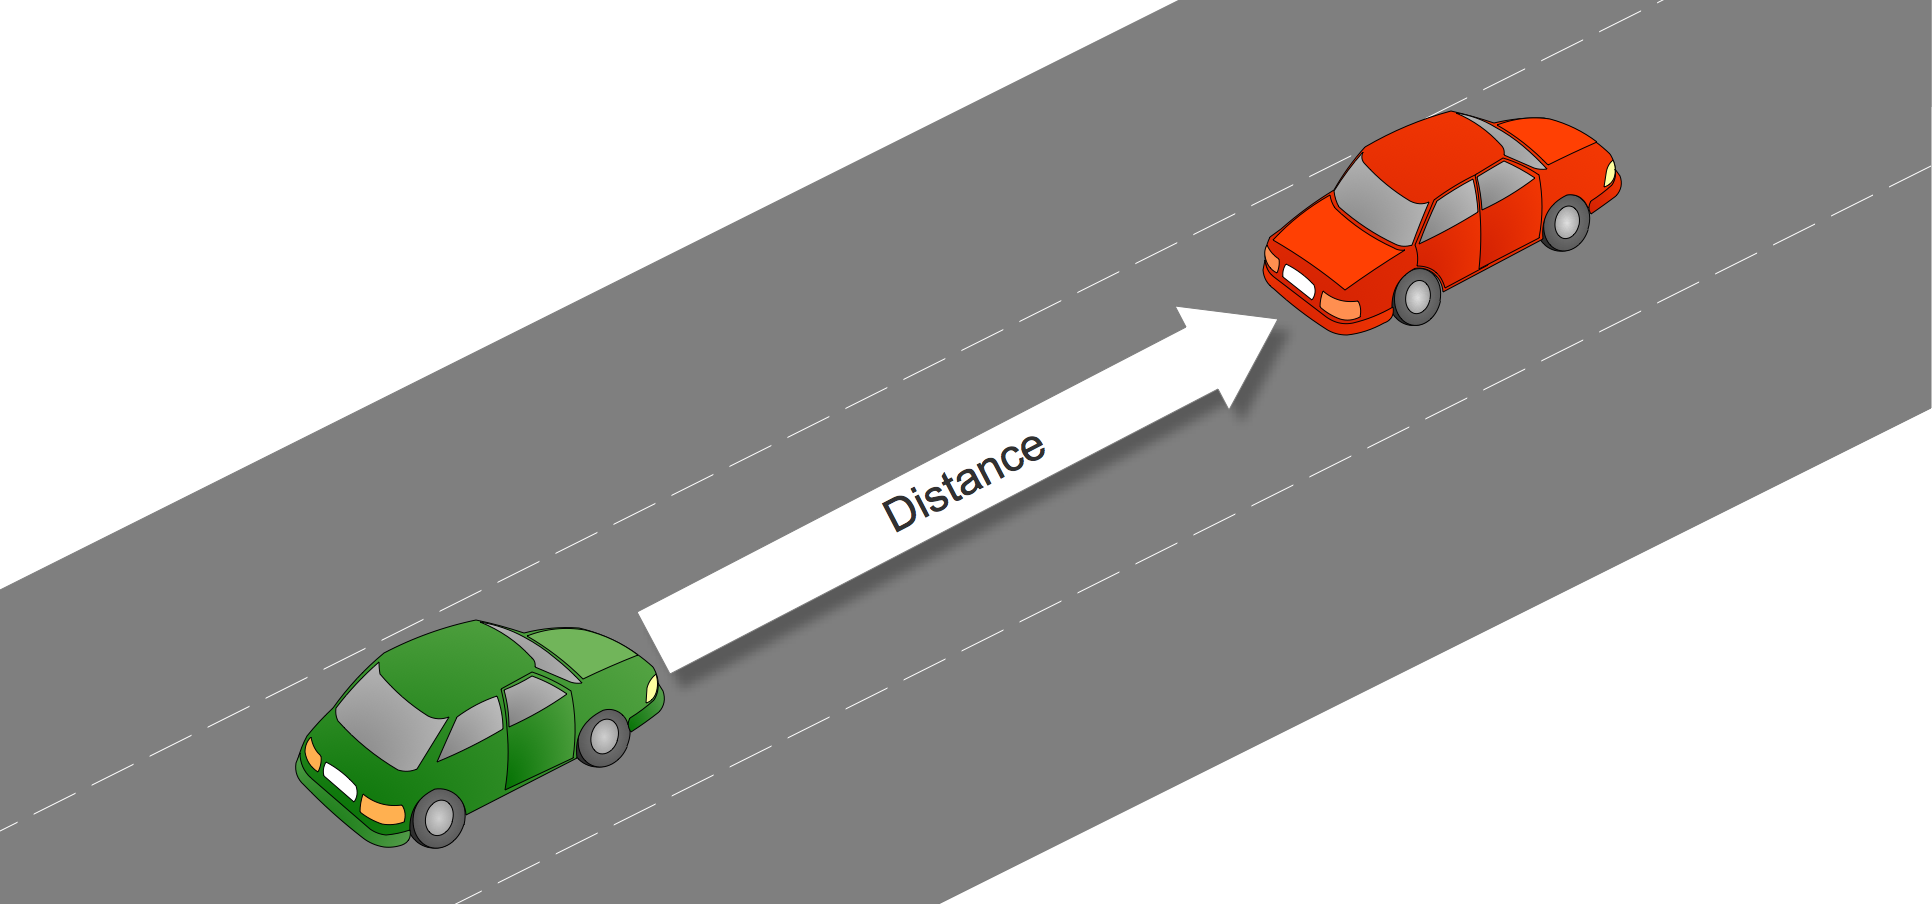
\includegraphics[width=0.45\textwidth]{text/figures/avgDistanceSameLane.png}}\\
    
    \subfloat[Other vehicle entering intersection - left turn across path.]{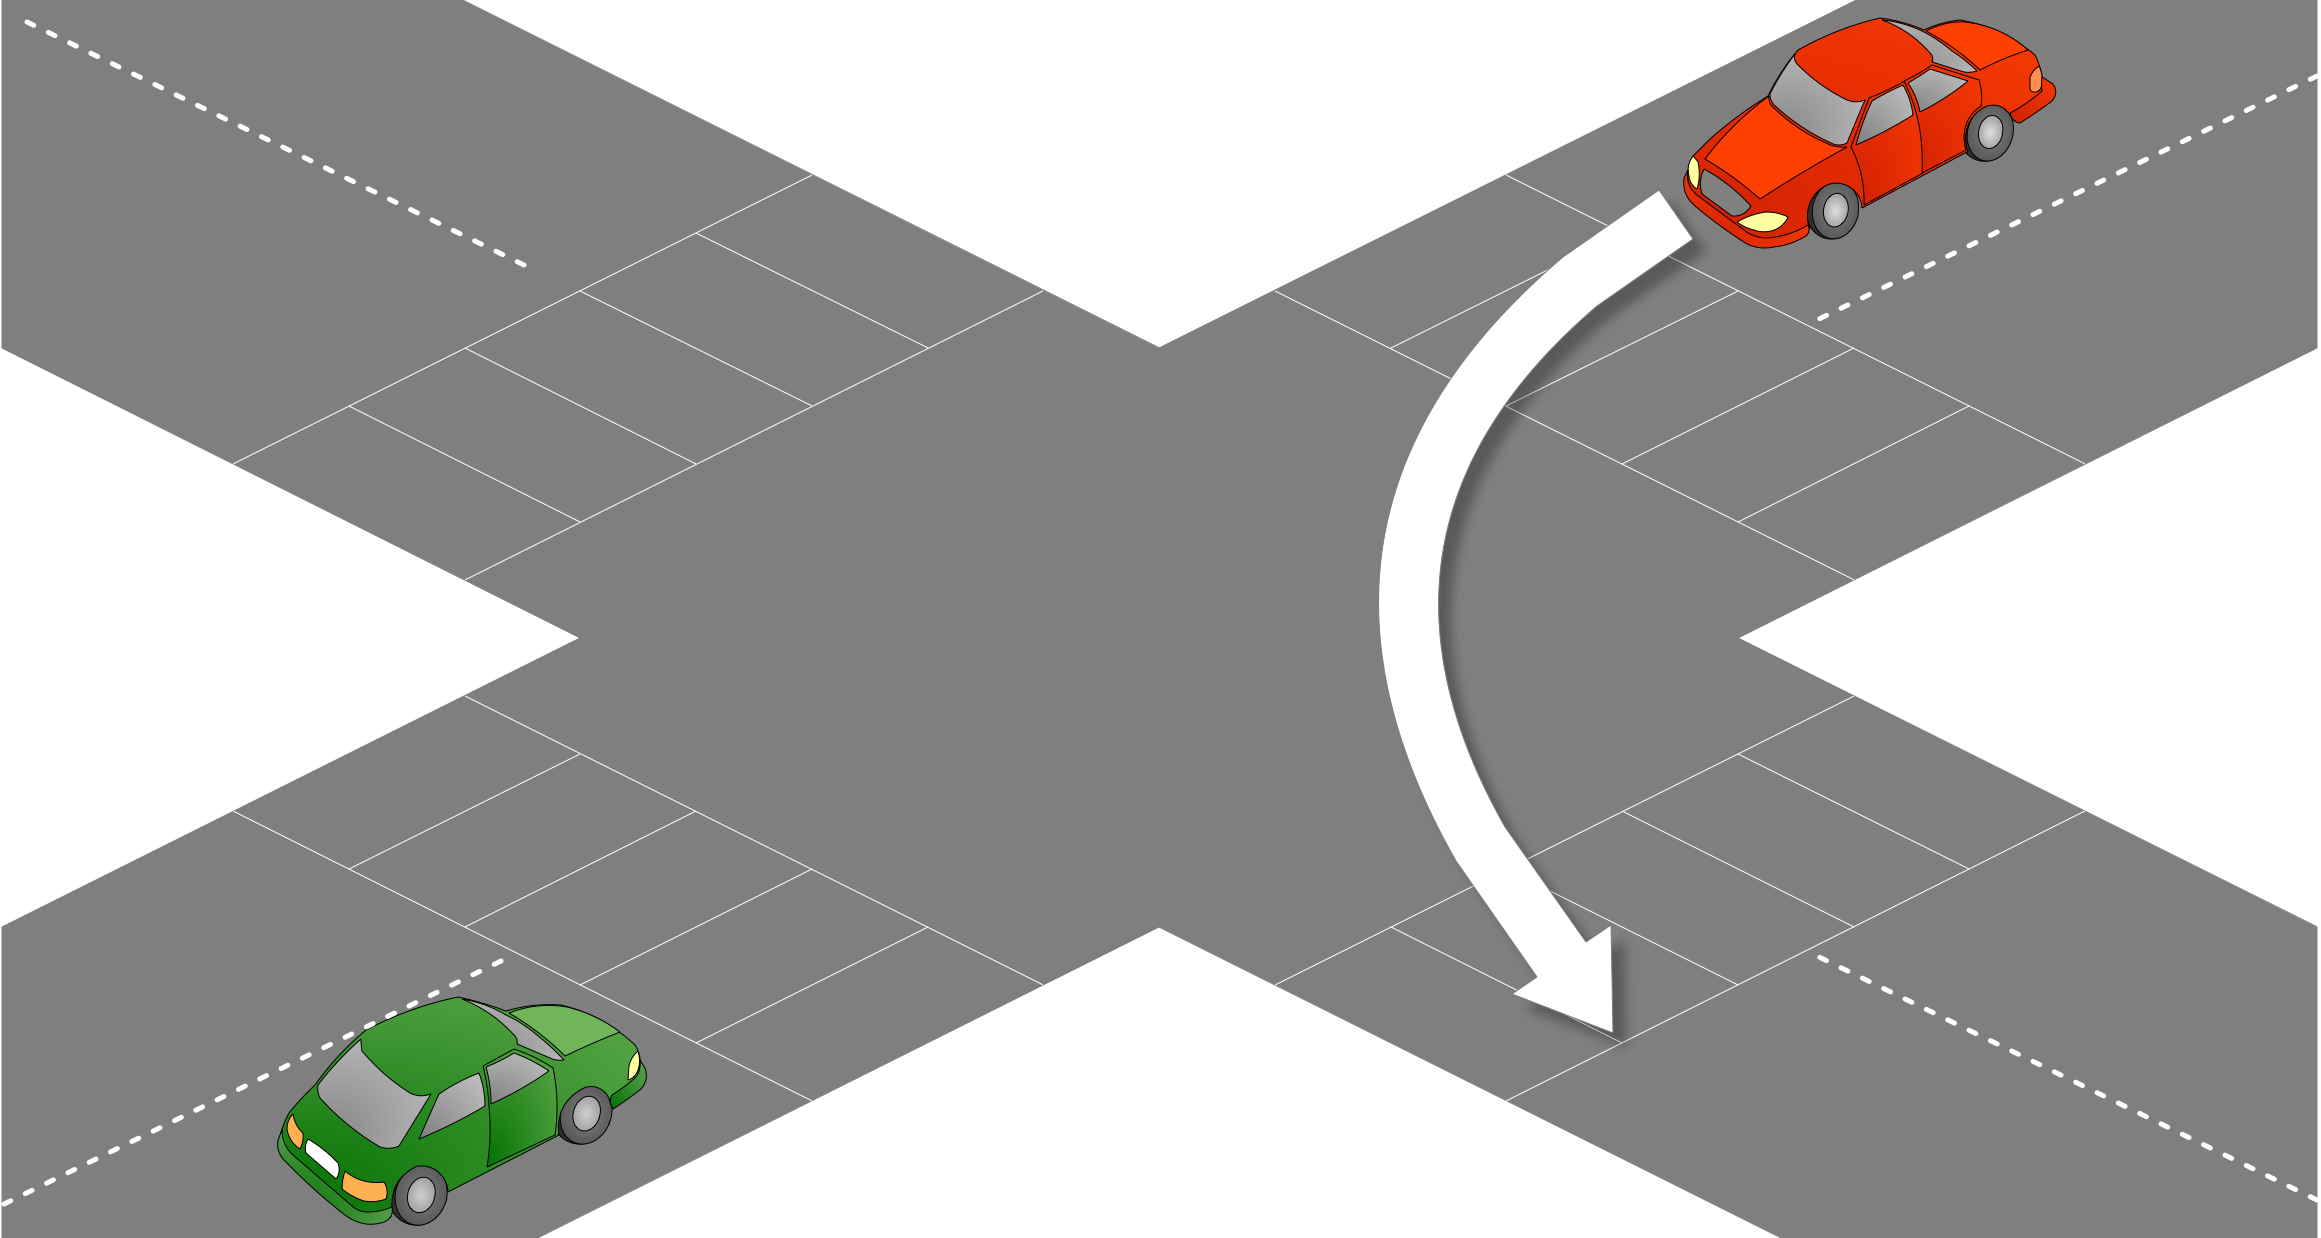
\includegraphics[width=0.45\textwidth]{text/figures/leftIntersect.png}} &
    \subfloat[Other vehicle entering intersection - turning onto opposite direction.]{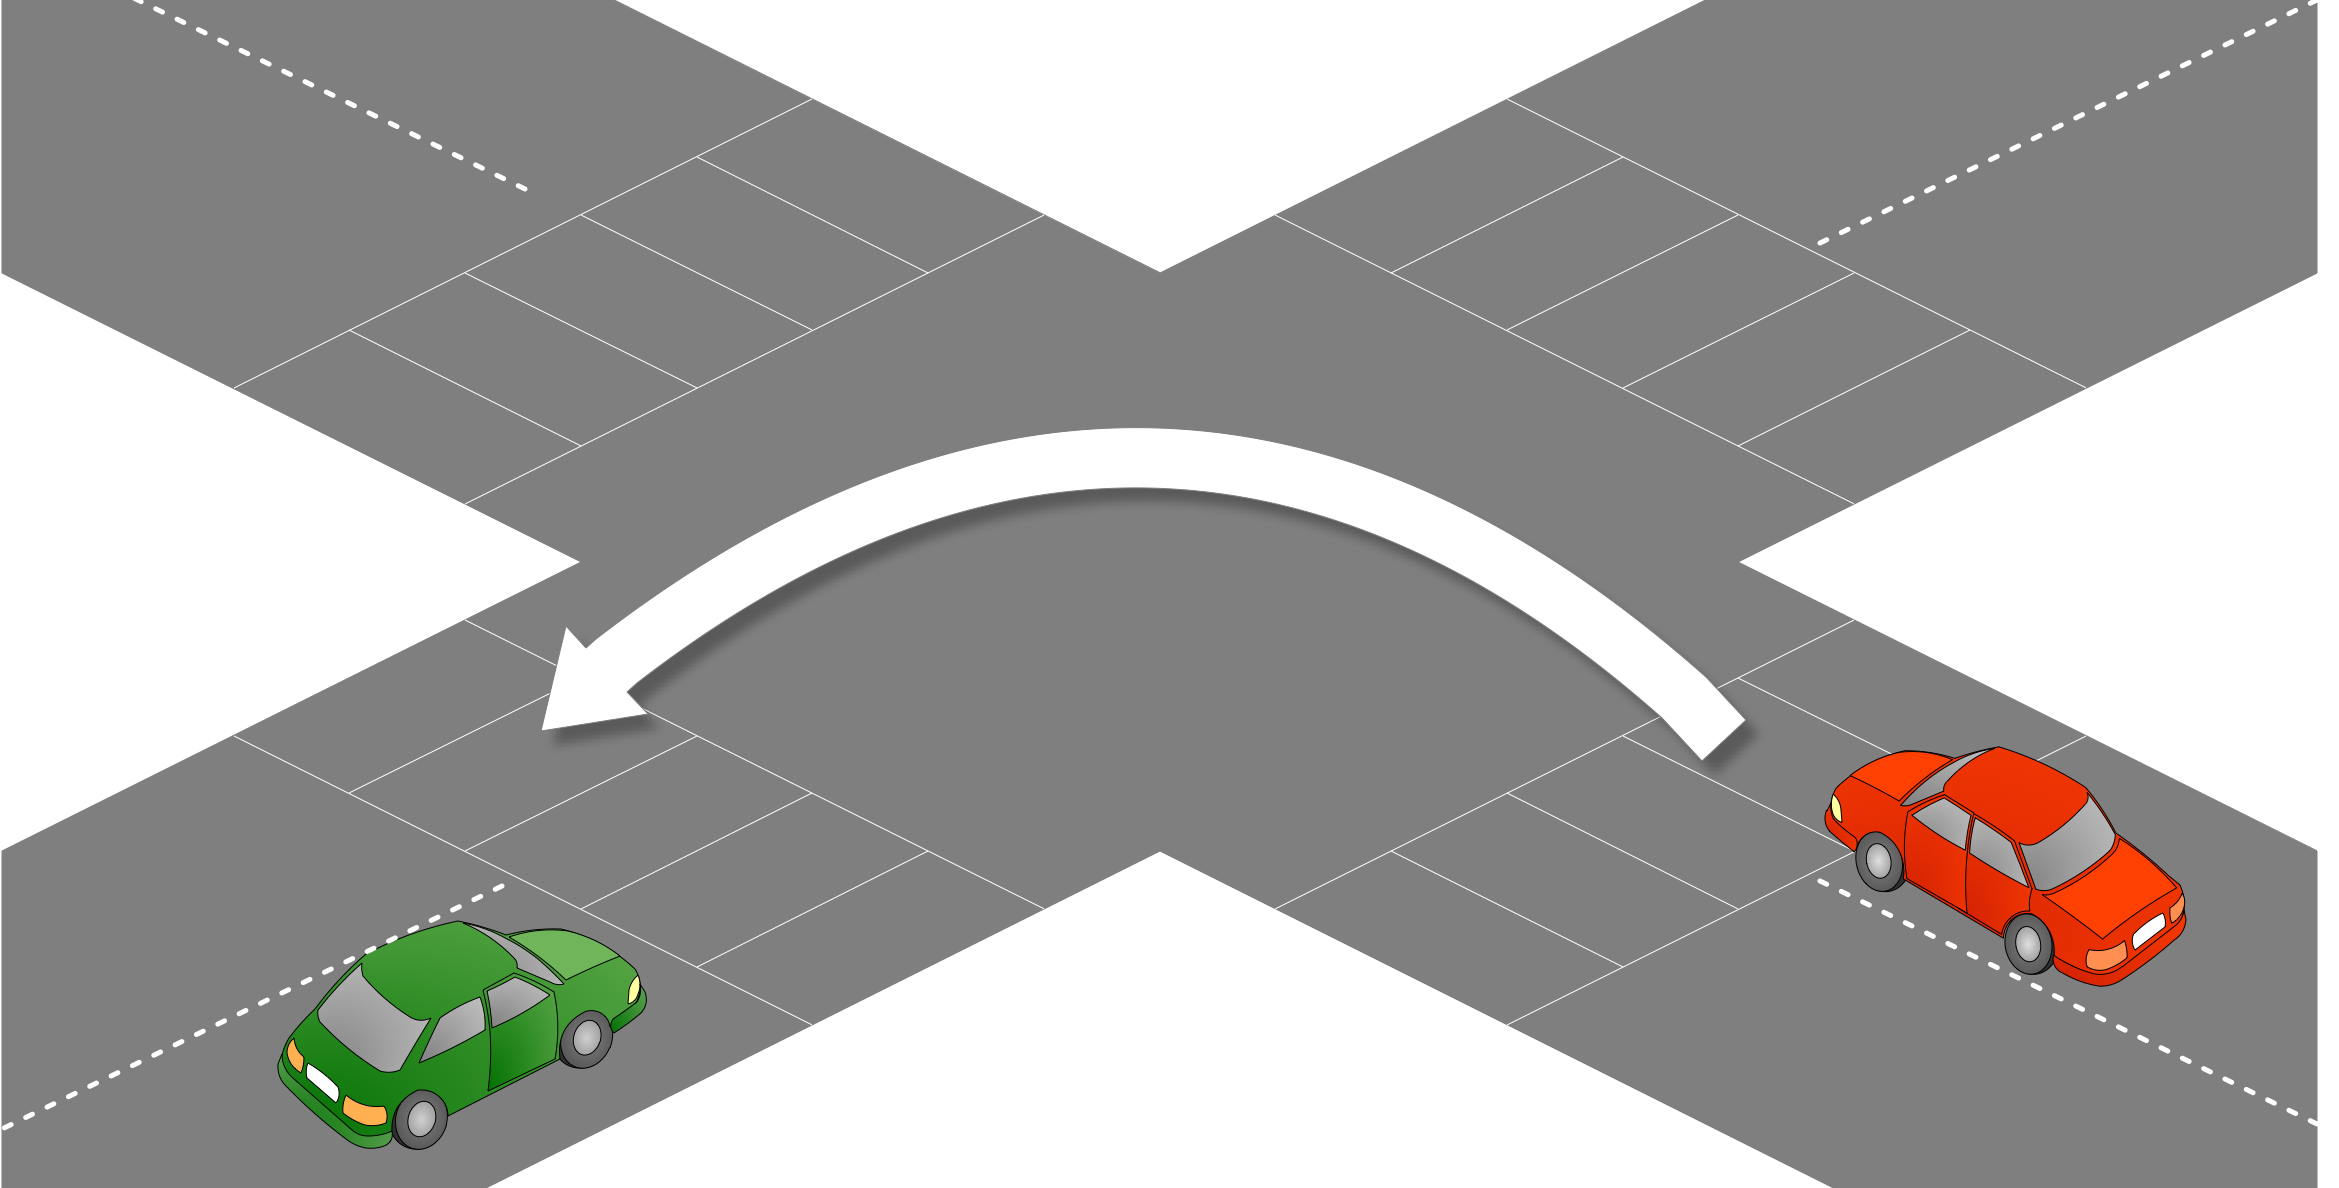
\includegraphics[width=0.45\textwidth]{text/figures/turningO.png}}\\
    
    \subfloat[Other vehicle entering intersection - straight across path.]{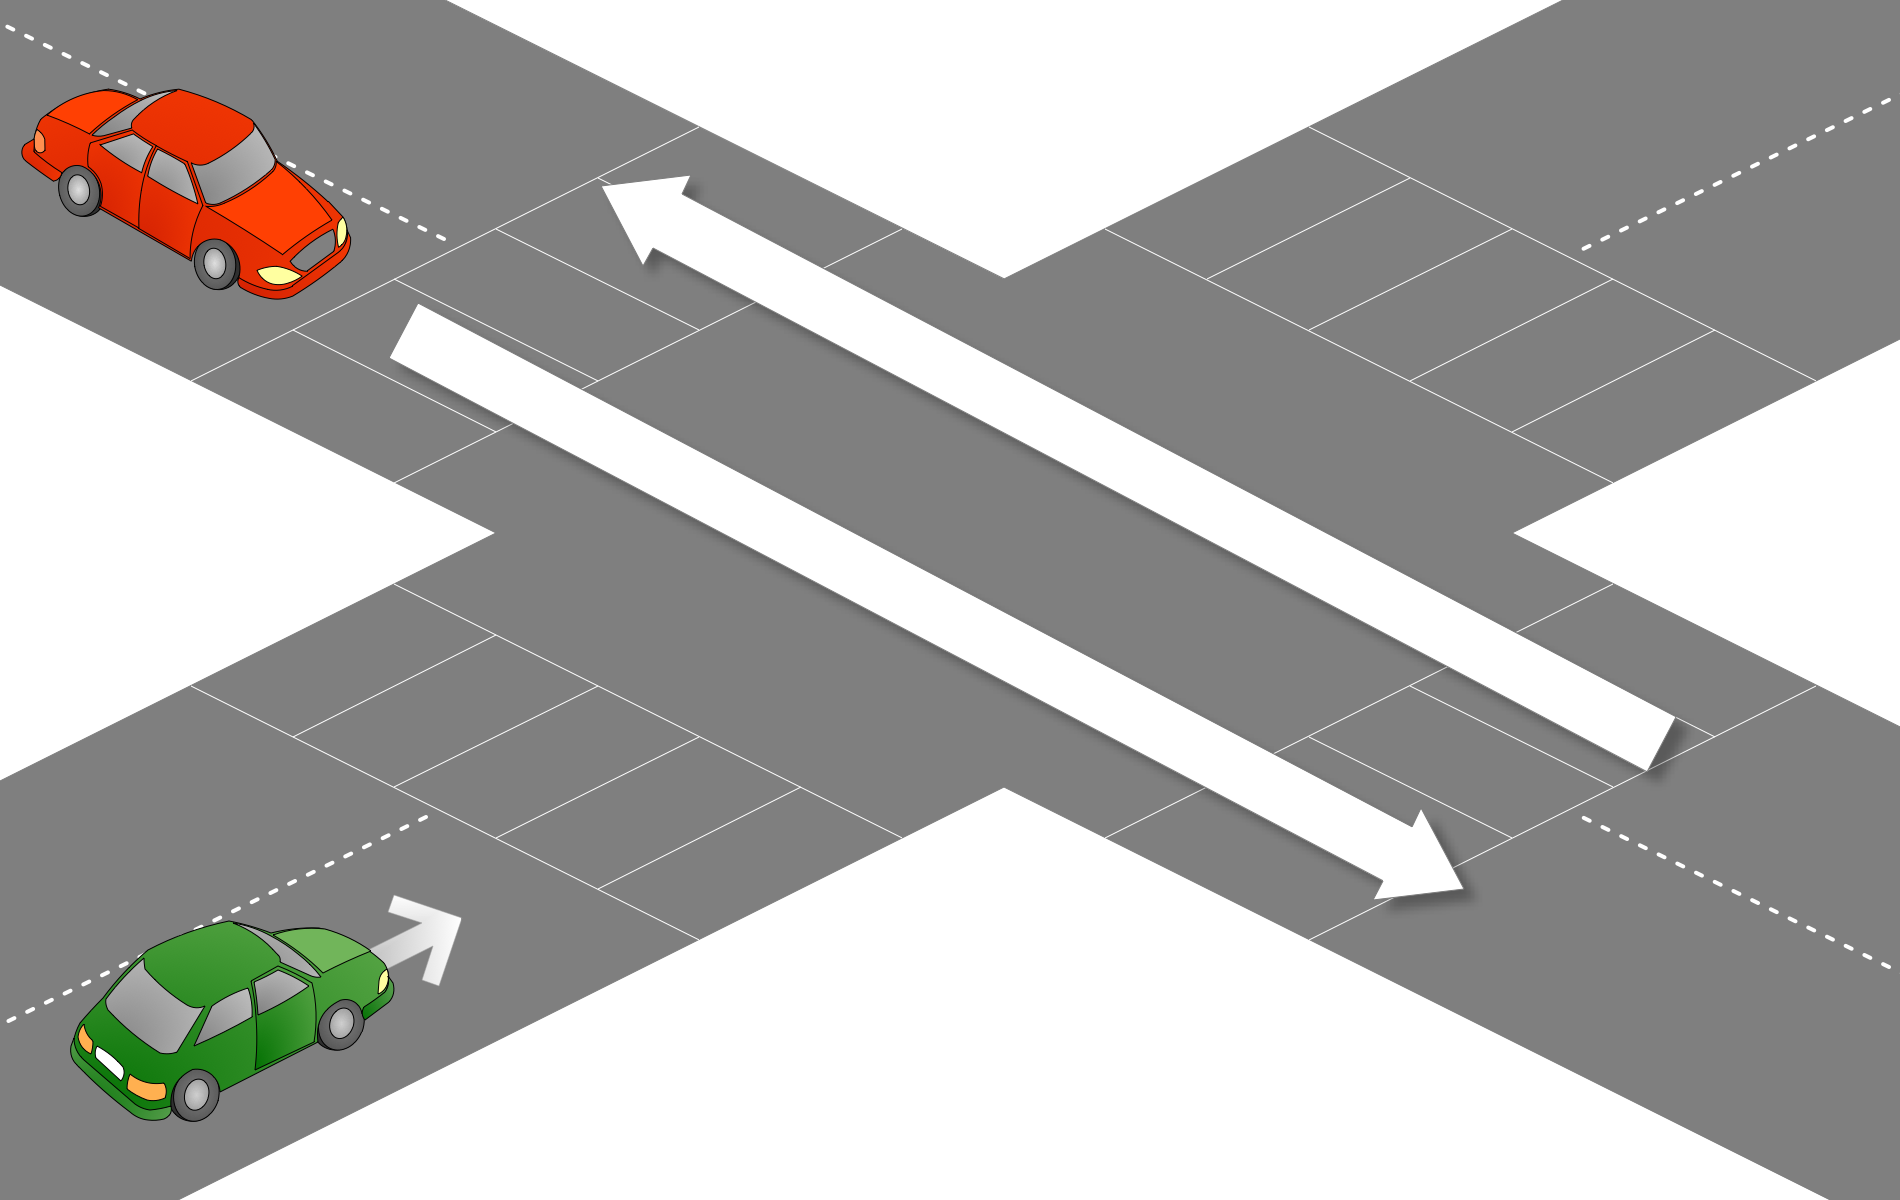
\includegraphics[width=0.45\textwidth]{text/figures/passingIntersect.png}} &
    \subfloat[Other vehicle entering intersection - turning same direction.]{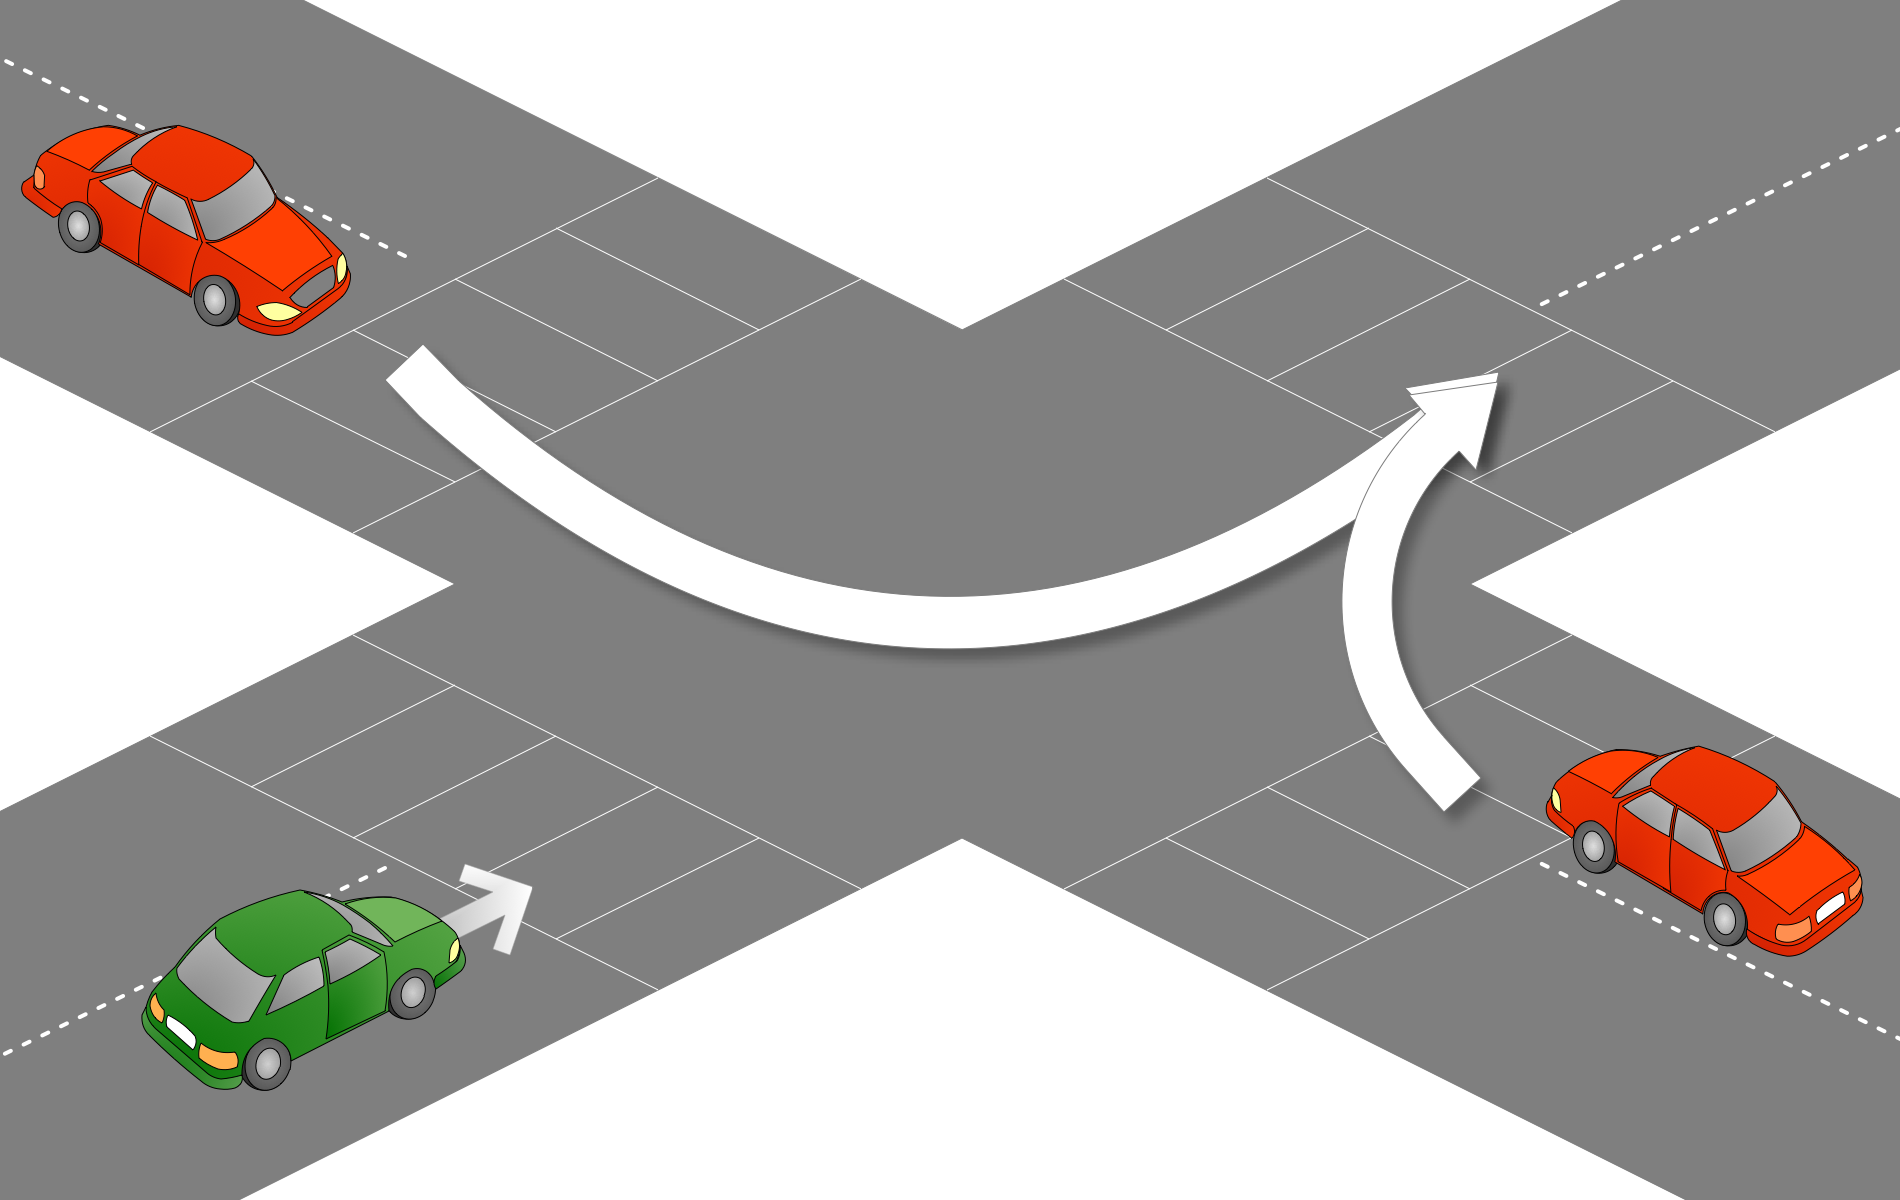
\includegraphics[width=0.45\textwidth]{text/figures/passingIntersectOntoSameDirection.png}}
  \end{tabular}
  \caption{Drive events that can be automatically detected by the method proposed in this paper. Green car is ego vehicle. Red cars are other vehicles. 
%(a) Average number of cars in front of ego-vehicle (b) Distance to rear-end of vehicle directly in front. (c) Other vehicle entering intersection - left turn across path (d) Other vehicle entering intersection - turning onto opposite direction (e) Other vehicle entering intersection - straight across path (f) Other vehicle entering intersection - turning same direction.
}
\end{figure}